\documentclass[11pt]{article}
\usepackage[a4paper,includeheadfoot,margin=2.54cm]{geometry}
% \usepackage{cmbright}
\usepackage[OT1]{fontenc}
\usepackage{graphicx}
% \usepackage{antiqua}
% \usepackage[T1]{fontenc}
% \usepackage{notomath}
\usepackage{parskip}

\begin{document}

\underline{\textbf{Atividade 10 - Trabalho prático}}\par
\textbf{Sistemas de Informação}\\
\textbf{Instituto Federal do Espírito Santo}\\
Campus Serra - Espírito Santo\par
\textbf{Teoria Geral de Sistemas}\\
Prof. Rodrigo Fernandes Calhau\par
Anderson A. Fraga (20222BSI0482)\\
\texttt{aafrg@tuta.io}\\  %\texttt formats the text to a typewriter style font

\textbf{- o que você fez (se possível enviar prints);}\par
Na última semana foram desenvolvidos os diagramas de fluxo e em níveis baseados no sistema elegido como representante como sistema sociotécnico - o caixa de supermercado.
\begin{figure}[!h]
    \centering
    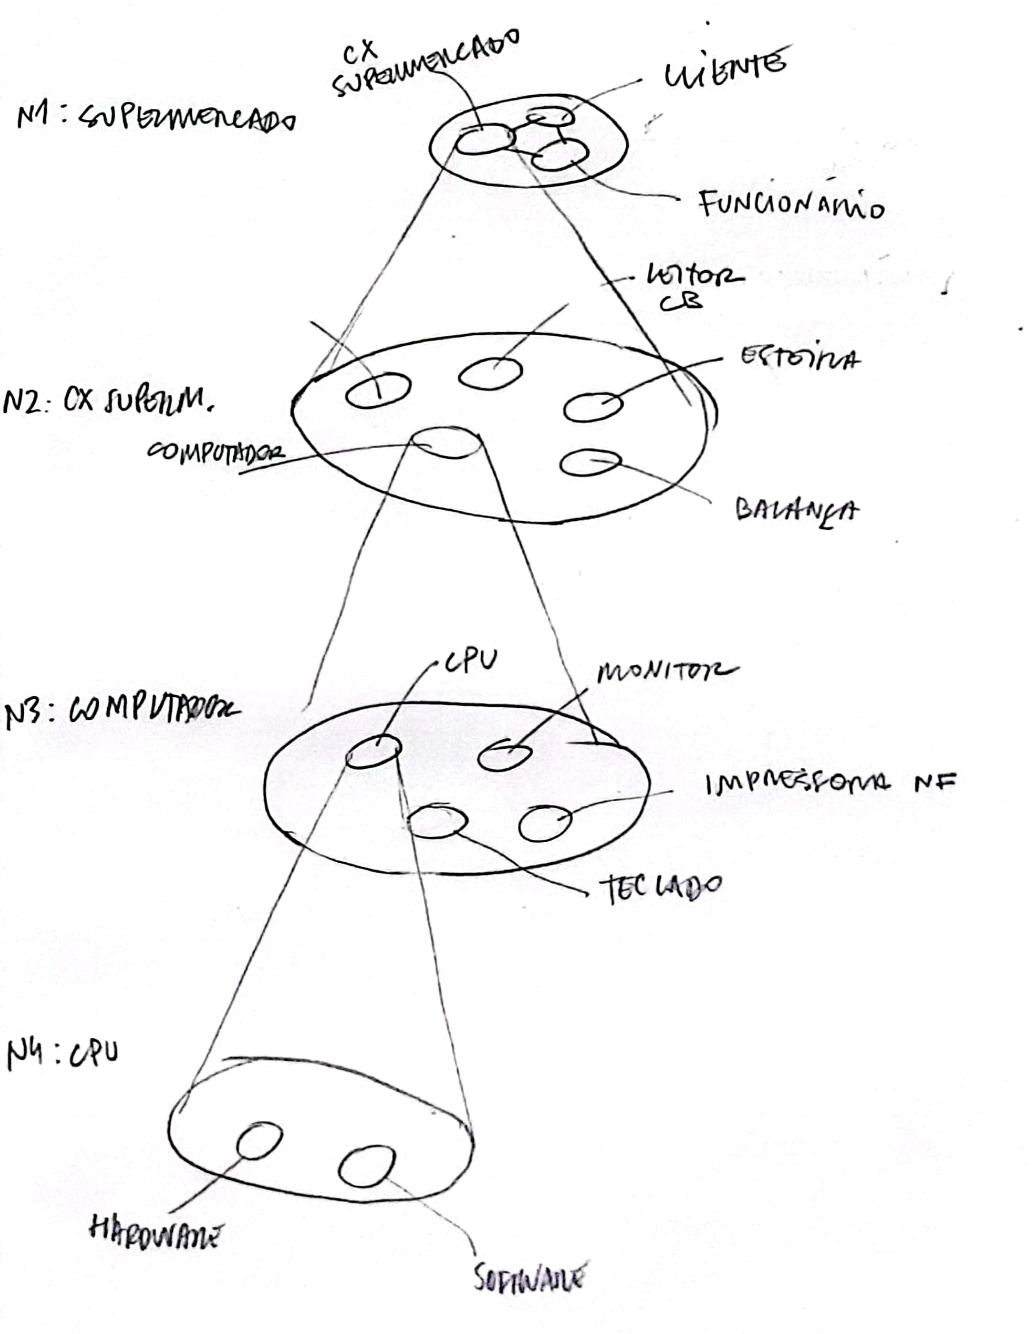
\includegraphics[width=8cm]{diagrama de niveis.PNG}
\end{figure}

\textbf{- quais dúvidas e impedimentos;}\par
Neste momento, as dúvidas estão relacionadas a como diferenciar os diagramas e mapas e em quais situações cada um se faz útil ou sobre sua aplicação específica. Após essa identificação, a implementação das ideias utilizando os diagramas tem sido rápida e clara.

\textbf{- quais os próximos passos;}\par
Estamos aguardando o início da etapa de modelagem de sistemas para aplicarmos no nosso estudo de caso escolhido.

\textbf{- o que o grupo fez;}\par
O grupo passa por uma fase de reestruturação, com a saída da Thielly, que trancou o curso, e com a ausência frequente do Arthur. Estamos buscando a melhor forma de seguir com as atividade - eu e Vivian - para concluirmos a atividade proposta.

\end{document}